% Basic LaTeX template for NE 204 lab report
\documentclass[11pt]{article}

%==============================================================================
%%% Everything between the "="'s is the preamble.
%%% Define packages and meta data here

% Common packages
\usepackage{amsmath}    % Expanded math
\usepackage{amssymb}    % Expanded math symbols
\usepackage{graphicx}   % For images
%\usepackage[version=3]{mhchem} % For nuclide formatting

% All images/figures will be stored in the images folder.
% Specify that here so pdflatex knows where to look for images.
\graphicspath{{./images/}}

% Metadata
\title{NE 204 Lab 0 - Energy Calibration with Reproducible Work
ows}
\author{Darrell Stepter}
\date{\today}
%==============================================================================

\begin{document}

% Compile metadata from preamble into a nicely-rendered title section
\maketitle

% The *'s next so section/subsection definitions suppresses numbering
\section*{Introduction}
\label{sec:intro}
The purpose of Lab0 is to practice generating lab reports using the reproducible work flow required for NE204: Advanced Concepts in Radiation Detection. Energy calibration of a High Purity Germanium (HPGe) detector, a ubiquitous task in radiation detection laboratories, was used for practicing the work flow. Energy calibration is a necessary step for every radiation detector. This is especially true for HPGe Detectors that are able to achieve high-energy resolution beyond what other detectors, such as scintillators, are capable of. Precise calibration ensures the accuracy and the quality of the results. Without a proper calibrations, there is no way to tell how the channels/bins from a Multi-Channel Analyzer (MCA) correlate to energy. In Lab0 this energy calibration was done using a two-point linear calibration between two gamma-ray photopeaks of $^{137}$Cs and $^{241}$Am. Subsequently, the calibration model was "verified" by applying it to a third gamma-ray photopeak from $^{133}$Ba. This report details the process and results of a two-point linear calibration.


\section*{Methods}
\label{sec:meth}
The data for this lab came from a HPGe detector collected by Dr. Ross Barnowski. The sources used to generate the spectrum are shown in Table \ref{tab:sources}.

\begin{table}[H]
\centering
\caption{Sources for Lab0}
\label{tab:sources}
\begin{tabular}{@{}lllll@{}}
\toprule
$^{241}$Am & $^{133}$Ba & $^{60}$Co & $^{137}$Cs & $^{152}$Eu \\ \bottomrule
\end{tabular}
\end{table}

The energy calibration was performed using a two-point linear fit between $^{137}$Cs and $^{241}$Am. To perform the calibration, a simple python peak detection script searched the raw spectrum data of $^{137}$Cs and $^{241}$Am looking for the channel containing largest number of counts (photopeak) within the spectrum. The program iterated over the spectrum by channel trying to identify a large delta (40000) in the counts. Because $^{137}$Cs and $^{241}$Am have single gamma ray photopeaks, a large delta ensures no other noise in the signal could be misconstrued as photopeaks.

Once the $^{137}$Cs and $^{241}$Am peaks were discovered, the python function polyfit was used to plot a linear line. The inputs to polyfit were the channel of the peak and the actual gamma-ray photopeak energy as listed in the IAEA Isotope Browser. The polyfit output was a slope and intercept that can be used to translate channel to energy. Next, the peak detection script was used to find the multiple photopeaks in the $^{133}$Ba sprectrum. Lastly, the polyfit "calibration" was applied to the $^{133}$Ba photopeaks and spectrum to calculate approximation error and display the full $^{133}$Ba spectrum.


\section*{Results}
\label{sec:res}
The peak detection script found the $^{241}$Am photopeak in channel 208 and the $^{137}$Cs photopeak in channel 2354. The documented energies for these photopeaks are 59.541 keV  and 661.657 keV, respectively. The identified photopeaks of $^{241}$Am and $^{137}$Cs are depicted in Figure \ref{fig:Peaks}.

\begin{figure}[H]
\centering
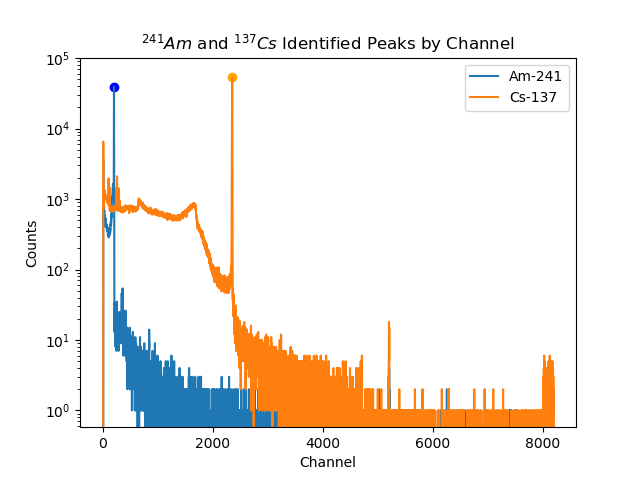
\includegraphics[scale=0.8]{images/Peaks.png}
\caption{Photopeaks of $^{241}$Am and $^{137}$Cs}
\label{fig:Peaks}
\end{figure}

The polyfit function found the linear relationship between channel and energy to be
\begin{align}
E_{calib} = 0.2805759552656106\cdot C + 1.1812013047530752 \label{eq:1}
\end{align}
where $E_{calib}$ is energy in keV and $C$ is channel number. Figure \ref{fig:Fit} depicts this linear calibration.

\begin{figure}[H]
\centering
\includegraphics[scale=0.8]{images/LinearFit.png}
\caption{Linear Fit of Channel to Energy}
\label{fig:Fit}
\end{figure}

The peak detection script found the $^{133}$Ba photopeaks in channels 13, 105, 284, 981, 1075, 1265, and 1364. However, the first two channels could be excluded from the data set because they are indicative of the 31 keV X-ray and the 80.9979 keV escape peak. Figure \ref{fig:BaPeaks} depicts the photopeaks found in $^{133}$Ba.

\begin{figure}[H]
\centering
\includegraphics[scale=0.8]{images/BaPeaks.png}
\caption{$^{133}$Ba Photopeaks}
\label{fig:BaPeaks}
\end{figure}

The photopeaks for $^{133}$Ba were calculated using Equation \ref{eq:1}. Figure \ref{fig:BaSpecCal} depict the calibrated $^{133}$Ba spectrum and Table \ref{tab:Comp} shows a comparison of the calibrated and known peak energies for $^{133}$Ba.

\begin{figure}[H]
\centering
\includegraphics[scale=0.8]{images/BaSpecCal.png}
\caption{$^{133}$Ba Photopeaks}
\label{fig:BaSpecCal}
\end{figure}

\begin{table}[H]
\centering
\caption{Comparison of Photopeaks for $^{133}$Ba}
\label{tab:Comp}
\begin{tabular}{@{}ll@{}}
\toprule
Expected (keV) & Calibrated (keV) \\ \midrule
80.9979 & 80.86477260 \\
276.3989 & 276.42621342 \\
302.8508 & 302.80035322 \\
356.0129 & 356.10978472 \\
383.8485 & 383.88680429 \\ \bottomrule
\end{tabular}
\end{table}

The approximation error between calibrated and known energy values were quantified by Equations \ref{eq:2}, \ref{eq:3}, and \ref{eq:4}.
\begin{align}
\epsilon =\left | E_{calib}-E_{known} \right | \label{eq:2}
\end{align}
\begin{align}
\eta = \frac{\left | E_{calib}-E_{known} \right |}{E_{known}} \label{eq:3}
\end{align}
\begin{align}
\delta = \frac{\left | E_{calib}-E_{known} \right |}{E_{known}}\cdot 100 \label{eq:4}
\end{align}

\begin{table}[H]
\centering
\caption{Approximation Error in Calibrated $^{133}$Ba Photopeaks}
\label{tab:error}
\begin{tabular}{@{}llll@{}}
\toprule
$\gamma$ Energy & Absolute Error $\epsilon$ & Relative Error $\eta$  & Percent Error $\delta$ (\%) \\ \midrule
80.9979               & 0.1331273998135174        & 0.0016435907574581241  & 0.1643590757458124          \\
276.3989              & 0.027313420317000237      & 9.881884593969163e-05  & 0.009881884593969163        \\
302.8508              & 0.05044678471557518       & 0.00016657306077968155 & 0.016657306077968153        \\
356.0129              & 0.09688471575043422       & 0.00027213821676246627 & 0.027213821676246627        \\
383.8485              & 0.038304287045889396      & 9.979011783526416e-05  & 0.009979011783526417        \\ \bottomrule
\end{tabular}
\end{table}


\section*{Discussion}
\label{sec:disc}
A linear energy calibration model for a coaxial HPGe detector was successfully produced using reproducible workflows. The accuracy of the calibration was determined by applying the model to the $^{133}$Ba dataset. While Knoll~\cite{knoll2010radiation} suggests using a polynomial fit, the approximation error between the calibrated and expected energies was insignificant; indicative of a very reliable model. The highest error, a $\delta$ of 0.164359(\%), occurred at the 80.9979 keV photopeak. This is likely due a large channel width creating an inability to discriminate between the 80.9979 keV and 79.6142 keV photopeaks in $^{133}$Ba.


% Bibliography
\bibliographystyle{plain}
% Refers to a bibtex file in the current dir named "references.bib"
\bibliography{references}

\end{document}
